\section{Bitcoin and Blockchains}\label{sec:bitcoin-preliminaries}

Blockchains are a special family of protocols that solve the distributed ledger
problem. Their name is derived from the mechanics of the underlying data
structure. Specifically, in blockchain systems, transactions are grouped in
blocks. Each block $\block$ contains an Merkle Tree~\cite{C:Merkle87} of
(ordered) transactions, as well as a hash pointer to another block. Each block
points to exactly one other block, thus forming a tree of blocks. The root of
the tree is typically a global parameter, called the ``genesis'' block. Each
branch of the tree consists of a well-ordered chain of blocks $\chain$, thus
implementing a distributed ledger (cf.
Section~\ref{subsec:distributed-ledger}). Additionally, a block contains a
timestamp and a nonce, which is used during the Proof-of-Work computation (see
below). Figure~\ref{fig:blockchain} depicts a simple model of Bitcoin's blocks.

\begin{figure}[h!]
	\centering
	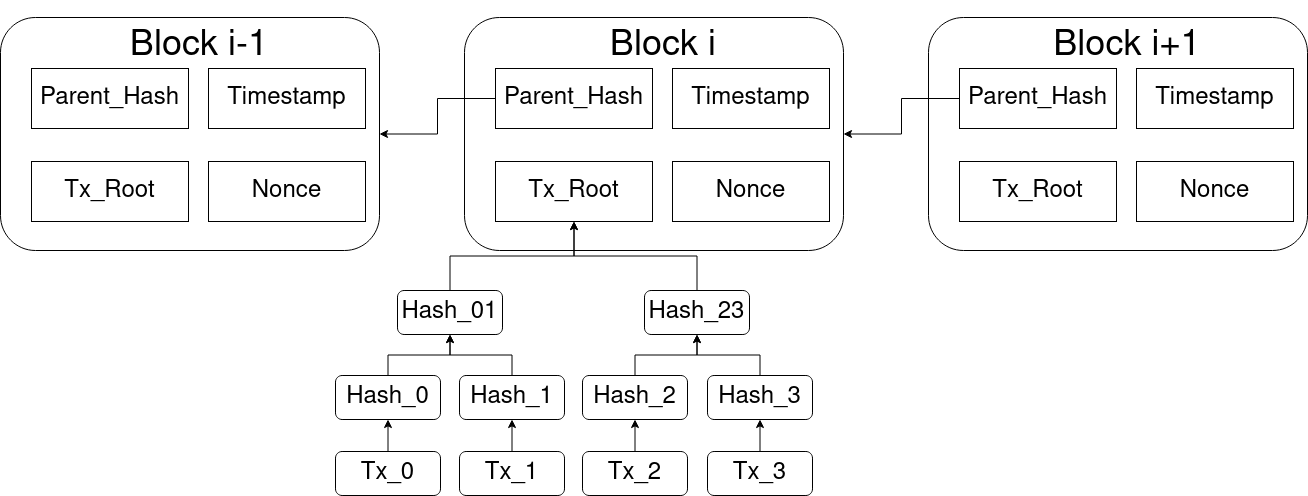
\includegraphics[width=1\columnwidth,keepaspectratio]{figures/blockchain.png}
	\caption{Bitcoin's blockchain data structure.}
	\label{fig:blockchain}
\end{figure}

For the rest of this thesis, we will use the following notation:
\begin{itemize}
    \item $\block$ denotes a block;
    \item $\chain$ denotes a chain of blocks;
    \item $\chain || \block$ denotes the concatenation of a chain and a block;
    \item $\head(\chain)$ denotes the last block of a chain $\chain$, \ie the
        block farthest from genesis \st $\head(\chain || \block) = \block$;
    \item ($\prec$) denotes the prefix operation between two chains; so, if
        $\chain' \prec \chain$, then there exists a chain of blocks $\block_0
        || \dots || \block_j$ such that $\chain = \chain' || \block_0 || \dots
        || \block_j$;
    \item ($\backslash$) denotes the difference of two chains, \eg if $\chain =
        \chain' || \chain''$ then $\chain'' = \chain \backslash \chain'$;
    \item $\chain^{\lceil k}$ denotes the chain obtained by removing the last
        $k$ blocks of chain $\chain$, \ie $\chain \backslash \chain^{\lceil
        k} = \chain'$ where $|\chain'| = k$;
    \item $|\chain|$ denotes the length of chain $\chain$ in blocks;
    \item $\chain[k]$ denotes either the $k$-th block or the $k$-th transaction
        in $\chain$ (depending on the context).
\end{itemize}

Bitcoin Backbone~\cite{EC:GarKiaLeo15,C:GarKiaLeo17} and
subsequently~\cite{EPRINT:KiaPan15} distilled the properties that a secure
blockchain protocol must satisfy (Definition~\ref{def:blockchain-extended}).
Based on these properties and Definition~\ref{def:secure-ledger},
Definition~\ref{def:blockchain} describes the combined, high-level properties
of \emph{persistence} and \emph{liveness} for blockchain-based distributed
ledgers.

\begin{definition}\label{def:blockchain-extended}
    Assume $\totalParties$ parties, each party $\party_i$ locally holding a chain
    $\chain_i = [\tx_{i, 0}, \dots, \tx_{i, j}]$. A secure blockchain protocol
    must satisfy the following properties:
    \begin{itemize}
        \item \emph{Common Prefix}: For parameters $\persistenceParam, \round_0
            \in \mbb{N}$, the chains $\chain_1, \chain_2$ held locally by the
            honest, but not necessarily distinct, parties $\party_1, \party_2$
            at rounds $\round_0 < \round_1 \leq \round_2$ respectively,
            satisfy: $\chain_1^{\lceil \persistenceParam} \prec \chain_2$.
        \item \emph{Chain Quality}: For parameters $l, \mu \in \mbb{N}$, any
            consecutive sequence of $l$ blocks, in a chain held locally by any
            honest party at any point in time, comprises of at least $\mu$
            blocks created by an honest party.
        \item \emph{Chain Growth}: For parameters $s, t \in \mbb{N}$, if at
            round $\round$ an honest party $\party_i$'s chain is
            $\chain_{i, \round}$, then, at round $\round + s$, the chain
            $\chain_{i, \round + s}$ locally held by $\party_i$ satisfies
            $|\chain_{i, \round + s}| \geq \chain_{i, \round} + t$.
    \end{itemize}
\end{definition}

\begin{definition}\label{def:blockchain}
    Assume $\totalParties$ parties, each party $\party_i$ locally holding a chain
    $\chain_i = [\tx_{i, 0}, \dots, \tx_{i, j}]$.

    We call a transaction $\tx$ \emph{stable} if, assuming that for some honest
    party $\party_i$ and some $k \in \mbb{N}$ it holds $\chain_i[k] = \tx$,
    then for every honest party $\party_l$ it holds $\chain_l[k] = \tx$.

    A blockchain-based distributed ledger protocol is secure, with parameters
    $\persistenceParam, \livenessParam$, if it satisfies the following properties:
    \begin{itemize}
        \item \emph{Persistence}:
            For each party $\party_i$, a transaction which is part of a block
            in a prefix chain $\chain_i' \prec \chain$, such that $|\chain_i| -
            |\chain_i'| \geq \persistenceParam$, is stable.
        \item \emph{Liveness}:
            A transaction which is provided as input to an honest party at
            round $\round$ has become stable by round $\round + \livenessParam$.
    \end{itemize}
\end{definition}

The major innovation of Bitcoin~\cite{nakamoto2008bitcoin} was to use a
blockchain to implement a secure distributed ledger under open and dynamic
participation~\cite{EC:GarKiaLeo15,C:GarKiaLeo17,EC:PasSeeShe17}. Up to that
point, distributed ledger
protocols assumed a known number of participating parties; instead, Bitcoin
allows parties to join or leave the protocol as needed. However, in such
open-participation setting, Bitcoin faced two questions: i) how to identify the
party responsible for producing a new block at any stage of the protocol; ii)
how to prevent sybil attacks~\cite{douceur2002sybil}. Briefly, in a sybil
attack an adversary creates a large number of pseudonymous identities to gain
disproportionate power in a system and subvert its security. Bitcoin answered
both these questions with its Proof-of-Work, with other blockchain protocols
following suit with alternatives like Proof-of-Stake.

\paragraph{Proof-of-Work (PoW)}
The core idea behind PoW~\cite{C:DwoNao92} is performing some amount of
computations and then, in order to participate in a protocol, publish a proof
of this ``work'' performed by the hardware. In cryptocurrencies like Bitcoin,
the PoW work is called ``mining''. The mining hardware is provided with two
constants, $\msf{previd}$ and $\msf{data}$, \ie the id of the tip of the
adopted blockchain and the data which need to be appended to it. The mining
device then brute-force searches for some string $\msf{nonce}$, such that
$\hash(\msf{previd} || \msf{data} || \msf{nonce}) \leq T$ for some hash
function $\hash$ defined by the system. $T$ is a --- relatively --- small
number, called the \emph{difficulty target}, which is adjusted to ensure a
stable block production rate, although typically remains constant for periods
of consecutive blocks called epochs. For example, in Bitcoin, epochs are $2016$
blocks long~\cite{SP:BMCNKF15}, while each new block is produced approximately
every $10$ minutes. Because the search for solutions is exhaustive, the
expected number of solutions found by a given miner is proportional to the
number of evaluations of the hash function $\hash$ they can obtain in a given
time frame.

\paragraph{Proof-of-Stake (PoS)}
PoW's deficiencies, particularly its egregious environmental cost, have driven research towards alternative designs,
most prominently Proof-of-Stake (PoS).  In PoS, a minter is selected in
proportion to the stake they hold, which is to say proportionally to the amount
of assets they own.  These assets are managed by the distributed ledger and
serve as both the system's internal currency and consensus participation
tokens.  There exist a number of flavors of this process. In one case, \eg
Ouroboros~\cite{C:KRDO17}, all coins automatically participate in the leader
election process. In a second flavour, the stake has to opt-in to participate
in the election by a special process, such as purchasing a ticket or becoming a
delegate of the stake of other users; this is the case for cryptocurrencies
like Decred~\cite{decred} and EOS~\cite{eosWhitepaper}. PoS systems are almost
energy-free, but often rely on complex cryptographic primitives, \eg secure
Multiparty Computation~\cite{C:KRDO17}, Byzantine
Agreement~\cite{FC:DaiPasShi19,DBLP:conf/sosp/GiladHMVZ17,USENIX:KJGKGF16}, or
Verifiable Random Functions (VRFs)~\cite{EC:DGKR18,DBLP:conf/sosp/GiladHMVZ17}.

Starting with Bitcoin, blockchain-based distributed ledgers are typically used
for financial applications. The ledger acts as a database which records the
ownership of digital assets at any point and the transactions, \ie transfers of
asset ownership, that are performed between users. Each user interacts with the
assets recorded on the ledger via \emph{addresses}.

An address $\addr$ is a string chosen from the set $\addresset \subseteq \{0,
1\}^\addrlen$, where $\addrlen$ is the --- protocol-specific --- address length
parameter. At any point in time, the ledger records the assets that each
address owns. A user controls a single \emph{account}, which may in turn
control multiple addresses; therefore, a user participates in the ledger, via
the account's addresses, in a pseudonymous manner.\footnote{The
literature has also seen a number of fully anonymous blockchain
protocols~\cite{SP:BCGGMT14,SP:MGGR13,EC:CGLMMM17,SP:KKKZ19}, but these are outside
the scope of this thesis.} Intuitively, an address is akin to an IBAN, in
traditional bank accounts. Typically, each address is associated with a payment
key pair $\keypair$, where $\pubkey$ is the public and $\privkey$ the private
key. As explored in Chapter~\ref{chap:delegation}, an address may be associated
with additional data, such as a staking key or metadata. Additionally, in
contract systems like Ethereum, a smart contract may not be associated with a
key pair, but rather only with a piece of software. However, in all cases,
addresses that are maintained by users of the system are associated with at
least one key pair, which is used for receiving and issuing payments.

To transfer assets between addresses, a user creates a transaction $\tx$. In
the simplest case, a transaction comprises of the following objects:
\begin{inparaenum}[i)]
    \item $\addr_s$: the address of the sender, \ie the current owner of the
        assets;
    \item $\addr_r$: the address of the receiver of the assets;
    \item $\asset$: the amount or set of assets which are transferred.
\end{inparaenum}
Typically, the transaction is also signed by the private key associated with
$\addr_s$, such that the sender can prove ownership of the assets. Optionally,
the transaction may also contain additional information, such as a number of
fees, a change address (\ie to receive surplus assets), or metadata (as
explored in Chapters~\ref{chap:hardware-wallets} and~\ref{chap:delegation}).
$\asset$ may be a simple number, if the exchanged assets are fungible, or a set
of individual asset identifiers, in the case of non-fungible assets.

\paragraph{Asset Fungibility}
An asset is fungible if each unit is indistinguishable from the others; in
contrast, each unit of a non-fungible asset is identified by a unique
identifier, which can be used to track it and trace its history. For example,
the US Dollar (USD) is a fungible asset, as citizens transact in amounts of USD
and each single unit of USD is indistinguishable. However, USD bills or
banknotes are non-fungible, since each bill is identified by a unique serial
number, which is often used to track forged or stolen assets. In our work, a
non-fungible asset is identified by a natural number $\asset$, while for
fungible assets we consider only amounts denoted by $\assetset$.
